\documentclass[serif,9pt]{beamer}
\usetheme{tree}
%\usepackage{german}
\usepackage[latin1]{inputenc}
\usepackage[spanish]{babel}

% Images
\usepackage{graphicx}
\usepackage{multicol} 
\usepackage{subfigure} % subfiguras
\usepackage{caption}
\usepackage{float}
\captionsetup[table]{labelformat=empty}
\captionsetup[figure]{labelformat=empty}

\usepackage{amsmath}

\usepackage{listings}
\lstset
{ %Formatting for code in appendix
  language=C++, % choose the language of the code
  basicstyle=\fontfamily{pcr}\selectfont\footnotesize\color{black},
  keywordstyle=\color{darkorange}\bfseries, % style for keywords
  numbers=left, % where to put the line-numbers
  numberstyle=\tiny, % the size of the fonts that are used for the line-numbers     
  backgroundcolor=\color{white},
  showspaces=false, % show spaces adding particular underscores
  showstringspaces=false, % underline spaces within strings
  showtabs=false, % show tabs within strings adding particular underscores
  tabsize=2, % sets default tabsize to 2 spaces
  captionpos=b, % sets the caption-position to bottom
  breaklines=false, % sets automatic line breaking
  breakatwhitespace=false, 
}

\AtBeginSection[]
{
  \begin{frame}<beamer>{Contenido}
    \tableofcontents[currentsection]
  \end{frame}
}

\definecolor{darkorange}{rgb}{0.94,0.4,0.0}

\begin{document}
\setbeamertemplate{navigation symbols}{}
\title{Cifrado con curvas el�pticas}  
\author{Yabir Garc�a Benchakhtir\\
David Cabezas Berrido\\
Patricia C�rdoba Hidalgo}
\date{}

\begin{frame}
\titlepage
\end{frame}

\section{Introducci�n}
\begin{frame}\frametitle{Introducci�n}
  Hablaremos de curvas el�pticas
\end{frame}

\section{Ejemplos}

\begin{frame}\frametitle{Ejemplos de curvas el�pticas}
\begin{figure}[H]
  \centering
\subfigure[Ejemplos de curvas el�pticas]{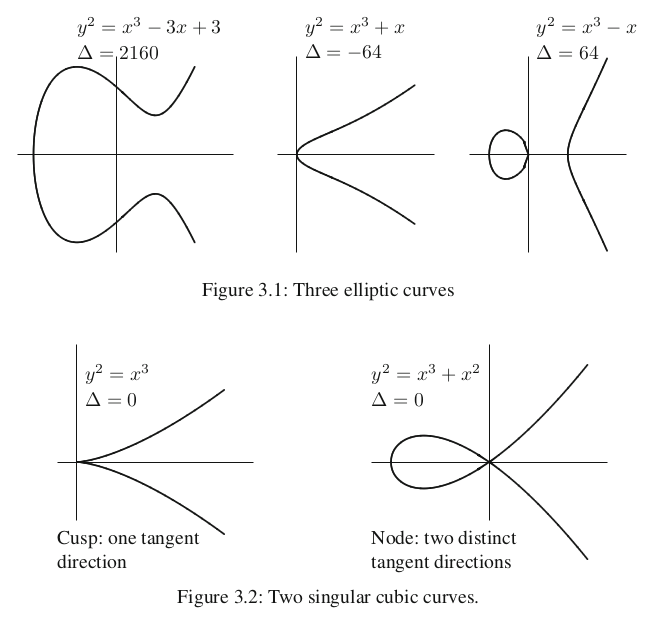
\includegraphics[width=70mm]{imagenes/curvas}}
\end{figure}
\end{frame}

\begin{frame}[fragile]\frametitle{Simulaci�n}
  \begin{lstlisting}
    Recuerda poner fragile en el c�gigo
  \end{lstlisting}
\end{frame}

\end{document}